\subsubsection{Historical Context and Evolution}
As outlined in the introductory section of the textbook \enquote{Artificial Intelligence: A Modern Approach} \cite{ai-modern-approach} \textemdash\ widely regarded as the standard text in the field \textemdash\ the development of artificial intelligence has been shaped by a series of major shifts in approach and methodology. 
In its early days, AI research was dominated by symbolic methods, which sought to represent knowledge and reasoning through explicit symbols and logical rules. 
These approaches aimed to model intelligent behavior by mimicking human reasoning processes.

Over time, researchers recognized the limitations of purely symbolic systems, especially when faced with the uncertainty and complexity of real-world environments. 
This realization led to the adoption of statistical and probabilistic methods, which allowed AI systems to learn from data and make decisions under uncertainty. 
The rise of machine learning marked a significant turning point, enabling computers to improve their performance through experience rather than relying solely on hand-crafted rules.

Another transformative phase in AI's evolution came with the development and resurgence of neural networks. 
Inspired by the structure of the human brain, neural networks provided a new way to process information and recognize patterns.

Advances in computational power and learning algorithms eventually led to the emergence of deep learning, which has driven remarkable progress in areas such as natural language processing and computer vision.%
\footnote{For comprehensive coverage of machine learning, specifically neural networks and deep learning architectures, see also \enquote{Deep Learning} by Goodfellow et al. \cite{deeplearning-book}, a foundational textbook on these topics}

Today, AI continues to evolve rapidly, integrating ideas from its symbolic, statistical, and neural network roots. 

\def\sectitle{Large Language Models}
\subsubsection%
[\sectitle]{\sectitle{} (LLMs) \cite{ai-modern-approach}}
LLMs represent the culmination of several decades of neural-network and deep-learning research.
To understand how they arose, it helps to contrast them with earlier sequence models, such as simple recurrent neural networks (RNNs).
RNNs process one token at a time and maintain a hidden state that is passed forward in time \textemdash\ a mechanism known as recurrence.
While they can in principle capture dependencies across a sequence, in practice they struggle with very long contexts and suffer from numerical underflow or overflow during training.

\paragraph{Tokens and Embeddings}  
LLMs operate on discrete units called tokens, which may be whole words, subwords, or characters, depending on the tokenization scheme.
Each token is converted into an embedding: a dense vector of floating-point numbers that encodes semantic and syntactic information.
Embeddings serve as the model's \enquote{language of thought}, allowing text symbols to be represented in a numerical form suitable for neural network architectures.

\paragraph{The Transformer Architecture}  
The transformer \cite{attention} replaces recurrence with a self-attention mechanism that allows every token to directly attend to every other token in a sequence.
Intuitively, self-attention computes a weighted sum of all token embeddings, where the weights reflect context-dependent relevance.
Transformers integrate multiple such attention blocks with simpler neural networks and stabilization mechanisms, enabling efficient, parallel modeling of long-range patterns.

\paragraph{Context and Context Size \cite{llm-survey}}
In LLMs, the context refers to the sequence of input tokens over which self-attention operates.
The context size (or context window) defines the maximum number of tokens the model can process simultaneously.
This size is typically determined during training and remains fixed for the model.
Context size is constrained by quadratic scaling of self-attention's computational and memory requirements.
Larger contexts enable longer-range dependencies and complex tasks like document summarization, but increase training and inference%
\footnote{Inference: The stage in which a trained model processes new inputs, i.e.\ its application after training
}
costs.

\paragraph{Pretraining, GPTs, and Fine-Tuning}  
Modern LLMs are often built on the GPT (Generative Pretrained Transformer) architecture \cite{gpt-family-paper}, which is a decoder-only transformer design.
This means they consist solely of the decoder stack from the original encoder-decoder design and therefore employ causal self-attention, ensuring each position attends only to earlier tokens.
During pretraining, GPT models learn to predict the next token in a text sequence. 
In this process, they acquire broad linguistic patterns from large-scale datasets, storing this knowledge in their parameters, the billions of numerical values that determine how inputs are transformed into generated outputs.

After pretraining, the resulting GPT foundation model can be fine-tuned on smaller, domain-specific datasets. 
This fine-tuning may involve updating all parameters or only specific layers, enabling the model to perform specialized tasks such as question answering or code generation.

\paragraph{Prompts and Few-/Zero-Shot Learning \cite{gpt3-paper}}  
A prompt is the natural-language text input provided to a LLM to specify a task or elicit a response.
A notable feature of GPT-style LLMs is their ability to follow prompts with little or no additional training.
In zero-shot mode, one supplies only an instruction, e.g.\ \enquote{Translate to French: ...}, and the model generates an answer directly.
In few-shot mode, several example input-output pairs are prepended to the prompt, allowing the model to infer the desired behavior.
These capabilities arise from extensive pretraining and the model's generalization of learned patterns to novel tasks.

\def\sectitle{Reasoning Models}
\subsubsection[\sectitle]{\sectitle{} \cite{reasoning-survey}}
Building on the foundations of pretraining, few-shot learning, and fine-tuning, a new class of models, often termed \emph{Reasoning Models}, has emerged to address fundamental limitations of standard LLMs. 
Standard large language models face several critical challenges when attempting reasoning tasks. 
They often hallucinate plausible but incorrect answers, struggle to decompose complex problems into manageable sub-problems, and exhibit brittle performance when reasoning chains exceed a few steps. 
Additionally, their predictions can be overly influenced by the frequency of certain terms in training data rather than logical reasoning processes, suggesting reliance on memorized patterns rather than true inference capabilities.

Reasoning models address these limitations through three key techniques:

\vspace{-1\baselineskip}
\paragraph{Chain-of-Thought (CoT) Prompting} 
By prompting models to \enquote{think step by step}, CoT elicits explicit intermediate rationales before producing final answers. 
This transforms single-shot predictions into sequential reasoning processes, significantly improving performance on arithmetic, logic, and commonsense benchmarks. 
Several variants have emerged: Zero-shot CoT uses simple prompts like \enquote{Let's think step by step} without examples, while rationale engineering techniques systematically improve the quality and effectiveness of reasoning demonstrations by optimizing how examples are constructed and selected.

\paragraph{Test-Time Scaling}
Unlike traditional scaling that increases model parameters, reasoning models dynamically allocate computational effort during inference (test time). 
Models learn to generate hundreds or thousands of reasoning tokens at test time, exploring multiple solution paths and self-correcting errors. 
This paradigm enables performance improvements through extended deliberation rather than larger model size.

\paragraph{Self-Correction and Verification}
Advanced reasoning models integrate self-consistency mechanisms that sample diverse reasoning chains and vote on consistent answers, alongside reflection processes that enable models to revisit and revise earlier reasoning steps when contradictions arise.

\paragraph{DeepSeek-R1 \cite{deepseekr1-report}} 
is a reasoning model developed by the Chinese AI company DeepSeek, exemplifying these principles through a multi-stage training approach.
The process begins with reinforcement learning applied to a base model (DeepSeek-R1-Zero) to develop reasoning behaviors. 
During this stage, the model learns through reward signals based on correctness, rather than supervised examples. 
This is followed by supervised fine-tuning with curated CoT data and iterative refinement through rejection sampling, a technique that generates multiple candidate responses and retains only the correct ones for training. 
This pipeline produces models capable of accurate and interpretable reasoning.

\vspace{\baselineskip}
These developments represent a shift from next-token prediction toward incentivized inference, where models are explicitly trained to deliberate, verify, and self-correct rather than merely mimic text patterns. 
However, current reasoning models still face significant limitations, including struggles with complex real-world reasoning tasks, sensitivity to prompt formulation, and the ongoing question of whether they perform genuine logical inference or sophisticated pattern matching. 
Despite these challenges, reasoning models mark an important step toward more capable AI systems for complex scientific and engineering applications.

\def\sectitle{Retrieval-Augmented Generation}
\subsubsection[\sectitle]{\sectitle{} \cite{rag-paper}}
Retrieval-Augmented Generation (RAG) addresses fundamental limitations of LLMs by combining their internal knowledge with external document collections for knowledge-intensive tasks.
Traditional language models store information in their parameters during training, making it difficult to update their knowledge or provide sources for their outputs.
RAG overcomes these challenges by retrieving relevant documents from an external corpus and using them as additional context during text generation.

The RAG approach consists of two main components: a retrieval system and a generation model.
Before any queries are processed, documents in the external corpus are indexed by converting them into vector embeddings and storing them in a searchable database.
During retrieval, the input query is similarly converted into an embedding and matched against the indexed documents to identify the most relevant passages.
The generation model then produces output based on both the original input and the retrieved context, combining parametric knowledge from training with non-parametric knowledge from the external corpus.

RAG offers two operational modes: one that uses the same retrieved documents for generating the entire output, and another that can select different documents for each part of the output.
This flexibility allows information synthesis from multiple sources when generating complex responses.

RAG demonstrates improved performance on knowledge-intensive tasks such as question answering, producing more factual outputs compared to standard language models.
A key advantage is the ability to update knowledge by replacing the document collection without retraining the model.
However, RAG introduces computational overhead and can be sensitive to retrieval quality, potentially producing errors when irrelevant information is retrieved.

\def\sectitle{Agentic AI}
\subsubsection[\sectitle]{\sectitle{} \cite{agent-paper}}
Agentic AI systems represent a paradigm shift from reactive language model responses toward autonomous, goal-directed artificial intelligence.
Unlike traditional LLMs that respond to individual prompts, agents exhibit goal-oriented behavior through sustained cycles of planning, execution, and adaptation.

\paragraph{Agent Architecture Components}
Modern agent architectures comprise several critical components enabling autonomous operation.
Planning modules decompose complex objectives into manageable subtasks and sequence actions toward goal completion.
Research identifies five major planning approaches: (1) task decomposition breaks problems into smaller sub-problems, (2) multi-plan selection evaluates multiple generated solution paths, (3) external module-aided planning leverages pre-existing external planners, (4) reflection and refinement revises plans based on new information, and (5) memory-augmented planning uses stored experiences to improve planning decisions.

Tool usage capabilities distinguish agents from standard language models by enabling interaction with external systems through function calling and API integration.
Using tools, agents can access databases, execute code, send emails, retrieve web content, and manipulate external environments, expanding their problem-solving scope beyond text generation.

Memory systems provide both short-term working memory for immediate context and long-term storage for accumulated experiences.

Reflection and learning mechanisms enable self-improvement through systematic evaluation of past actions and outcomes, reducing errors and improving decision-making quality over time.

\paragraph{Multi-Agent Systems and Coordination}
Multi-agent architectures extend individual capabilities through collaborative problem-solving, organizing specialized agents into coordinated teams for parallel task execution.
Two primary structures emerge: vertical architectures with leadership hierarchies and horizontal architectures emphasizing peer collaboration.

Effective systems employ structured communication protocols to prevent unproductive interactions and ensure relevant information reaches appropriate team members.
Multi-agent systems have proven successful in scenarios requiring diverse perspectives or collaborative decision-making, though they introduce coordination overhead.
Dynamic team formation, where agents are recruited based on task requirements, optimizes performance for specific problem phases.

\def\sectitle{Real-World Application: GitHub Copilot}
\subsubsection[\sectitle]{\sectitle{} \cite{copilot-product-page}\cite{copilot-docs}}

GitHub Copilot represents a prominent real-world implementation of the AI paradigms discussed previously, demonstrating how LLMs, retrieval-augmented generation, and agentic systems converge in practical software development tools.

Originally built upon OpenAI's Codex model \cite{codex-paper}, a specialized variant of GPT fine-tuned on publicly available code repositories, Copilot has evolved into a comprehensive AI-powered coding assistant developed by GitHub in collaboration with OpenAI.\footnote{%
    OpenAI: US-based AI research company, backed by Microsoft but operates independently; pioneer in modern LLMs, introducing the GPT architecture \cite{gpt-family-paper}\\
    GitHub: Platform for version control and collaborative software development; acquired by Microsoft in 2018.
}

\vspace{-0.8\baselineskip}
\paragraph{Hybrid Approach Integration}
GitHub Copilot embodies the hybrid AI approaches outlined in previous sections.
Its RAG components manifest through code repository indexing, where the system maintains awareness of project structure, dependencies, and coding patterns specific to the current workspace.
This contextual retrieval ensures suggestions better align with existing codebase conventions and architectural decisions.

Agentic features are evident in Copilot's ability to perform multistep tasks such as debugging workflows, where the system can analyze error messages, identify potential causes, and suggest comprehensive fixes.
The chat interface supports complex problem-solving scenarios, allowing developers to engage in iterative refinement of solutions through natural language dialogue.

The integration of reasoning capabilities appears in Copilot's code logic verification and optimization suggestions, where the system can evaluate code quality, identify potential improvements, and explain the rationale behind its recommendations.

\vspace{-0.8\baselineskip}
\paragraph{Performance and Limitations}
While GitHub Copilot has achieved widespread adoption\footnote{
    According to a recent press statement by Microsoft, more than 20 Million all-time users \cite{copilot-user-count}
}, it faces inherent limitations characteristic of current AI systems.
Code quality varies significantly depending on task complexity, with simpler, well-established programming patterns receiving more reliable suggestions than novel or domain-specific implementations.

Security considerations remain important, as the system may inadvertently suggest code patterns that introduce vulnerabilities or expose sensitive information.
Various safeguards have been implemented, including content filtering and bias detection mechanisms, but human oversight remains essential.

\def\sectitle{Visual Studio Code and the GitHub Copilot Extension}
\subsubsection[\sectitle]{\sectitle}

\paragraph{Visual Studio Code}
For source code editing tasks throughout this bachelor's thesis, I primarily used Microsoft's Visual Studio Code (VS Code) \cite{vscode} due to its user-friendly interface and my prior familiarity with the environment.
Additionally, it offers a wide range of useful extensions, such as the Remote Development Extension Pack \cite{vscode-remote}, which allows connecting to remote VS Code servers via SSH, and accessing most of the functionality of the editor as if working on a local machine, even if operating systems differ between the client and host.

While GitHub Copilot is available in a limited form on GitHub itself, it is primarily used as an extension within integrated development environments (IDEs). 
GitHub Copilot is particularly well integrated into Visual Studio Code through dedicated extensions \cite{vscode-copilot-extension}\cite{vscode-copilot-chat-extension}, which can be attributed to GitHub and VS Code both being Microsoft products.

As of late 2024, Copilot users can select from multiple language models, representing a significant change from earlier versions that used predetermined OpenAI GPT variants exclusively \cite{copilot-llm-select}. 
This flexibility allows developers to choose models based on their specific task requirements, with options ranging from fast completion-focused models to more sophisticated reasoning-oriented variants.

The VS Code extension implements GitHub Copilot through several key interfaces:

\vspace{-1\baselineskip}
\paragraph{The Copilot Panel} serves as the primary interaction hub and features a chat window that enables natural language communication with the AI system.
This chat interface operates in three distinct modes: Ask mode for exploratory queries and code explanations, Edit mode for direct multi-file modifications, and Agent mode for autonomous task execution.

The panel supports extensive context integration through various mechanisms: Users can reference the entire codebase, target specific files, folders or symbol definitions, and utilize specialized tools such as web content fetching capabilities (cf.\ Fig.\ \ref{fig:copilot-ui}, Right).

\vspace{-0.8\baselineskip}
\paragraph{Code Completion}
Beyond the panel interface, the extension provides real-time code completion suggestions that appear as developers type.
These suggestions range from single-line completions to entire function implementations based on contextual analysis of the surrounding code (see Fig.\ \ref{fig:copilot-ui}, Left).

\vspace{-0.8\baselineskip}
\paragraph{Inline Chat}
Inline chat functionality extends this interactivity directly into the editing environment, allowing developers to request code modifications or explanations without leaving their current file context.
This capability also extends to terminal integration, where users can invoke Copilot assistance for command-line tasks and debugging scenarios.

Beyond these core features, the GitHub Copilot extension offers numerous additional capabilities that I did not have the opportunity to explore in detail for this thesis.
The extension's ecosystem is expanding rapidly through frequent feature additions. 
These new capabilities include autonomous coding workflows, multistep task execution, and integration with external tools via the Model Context Protocol \cite{model-context-protocol}. 
This accelerated development reflects the broader trend of continuous innovation in AI-powered development tools.

\vspace{-0.8\baselineskip}
\paragraph{Choice of GitHub Copilot for Software Optimization Testing}
During the research phase of this thesis, I selected GitHub Copilot as the primary tool to test AI's capabilities in software optimization tasks.
This choice was driven by several considerations:

Since my development work was mainly conducted within VS Code, GitHub Copilot presented an easy integration into my familiar environment. 
This proved particularly valuable given the rapidly evolving landscape of AI development tools, where new products are released frequently, making it difficult to systematically evaluate all available options.

From a practical perspective, GitHub's Student Developer Pack \cite{github-student-dev-pack} currently provides free access to the Copilot Pro plan. 
This plan includes unlimited code completions and chat interactions with a subset of available models (\emph{Standard Models}), plus 300 monthly requests to the Pro tier's \emph{Premium Models}.\footnote{%
\textbf{Notes:}\\
- Based on my observations, one request equals one sent chat message\\
- For a list of all the models available in the Pro tier cf.\ section \ref{sec:model-selection}
}

\begin{figure}[h]
    \centering
    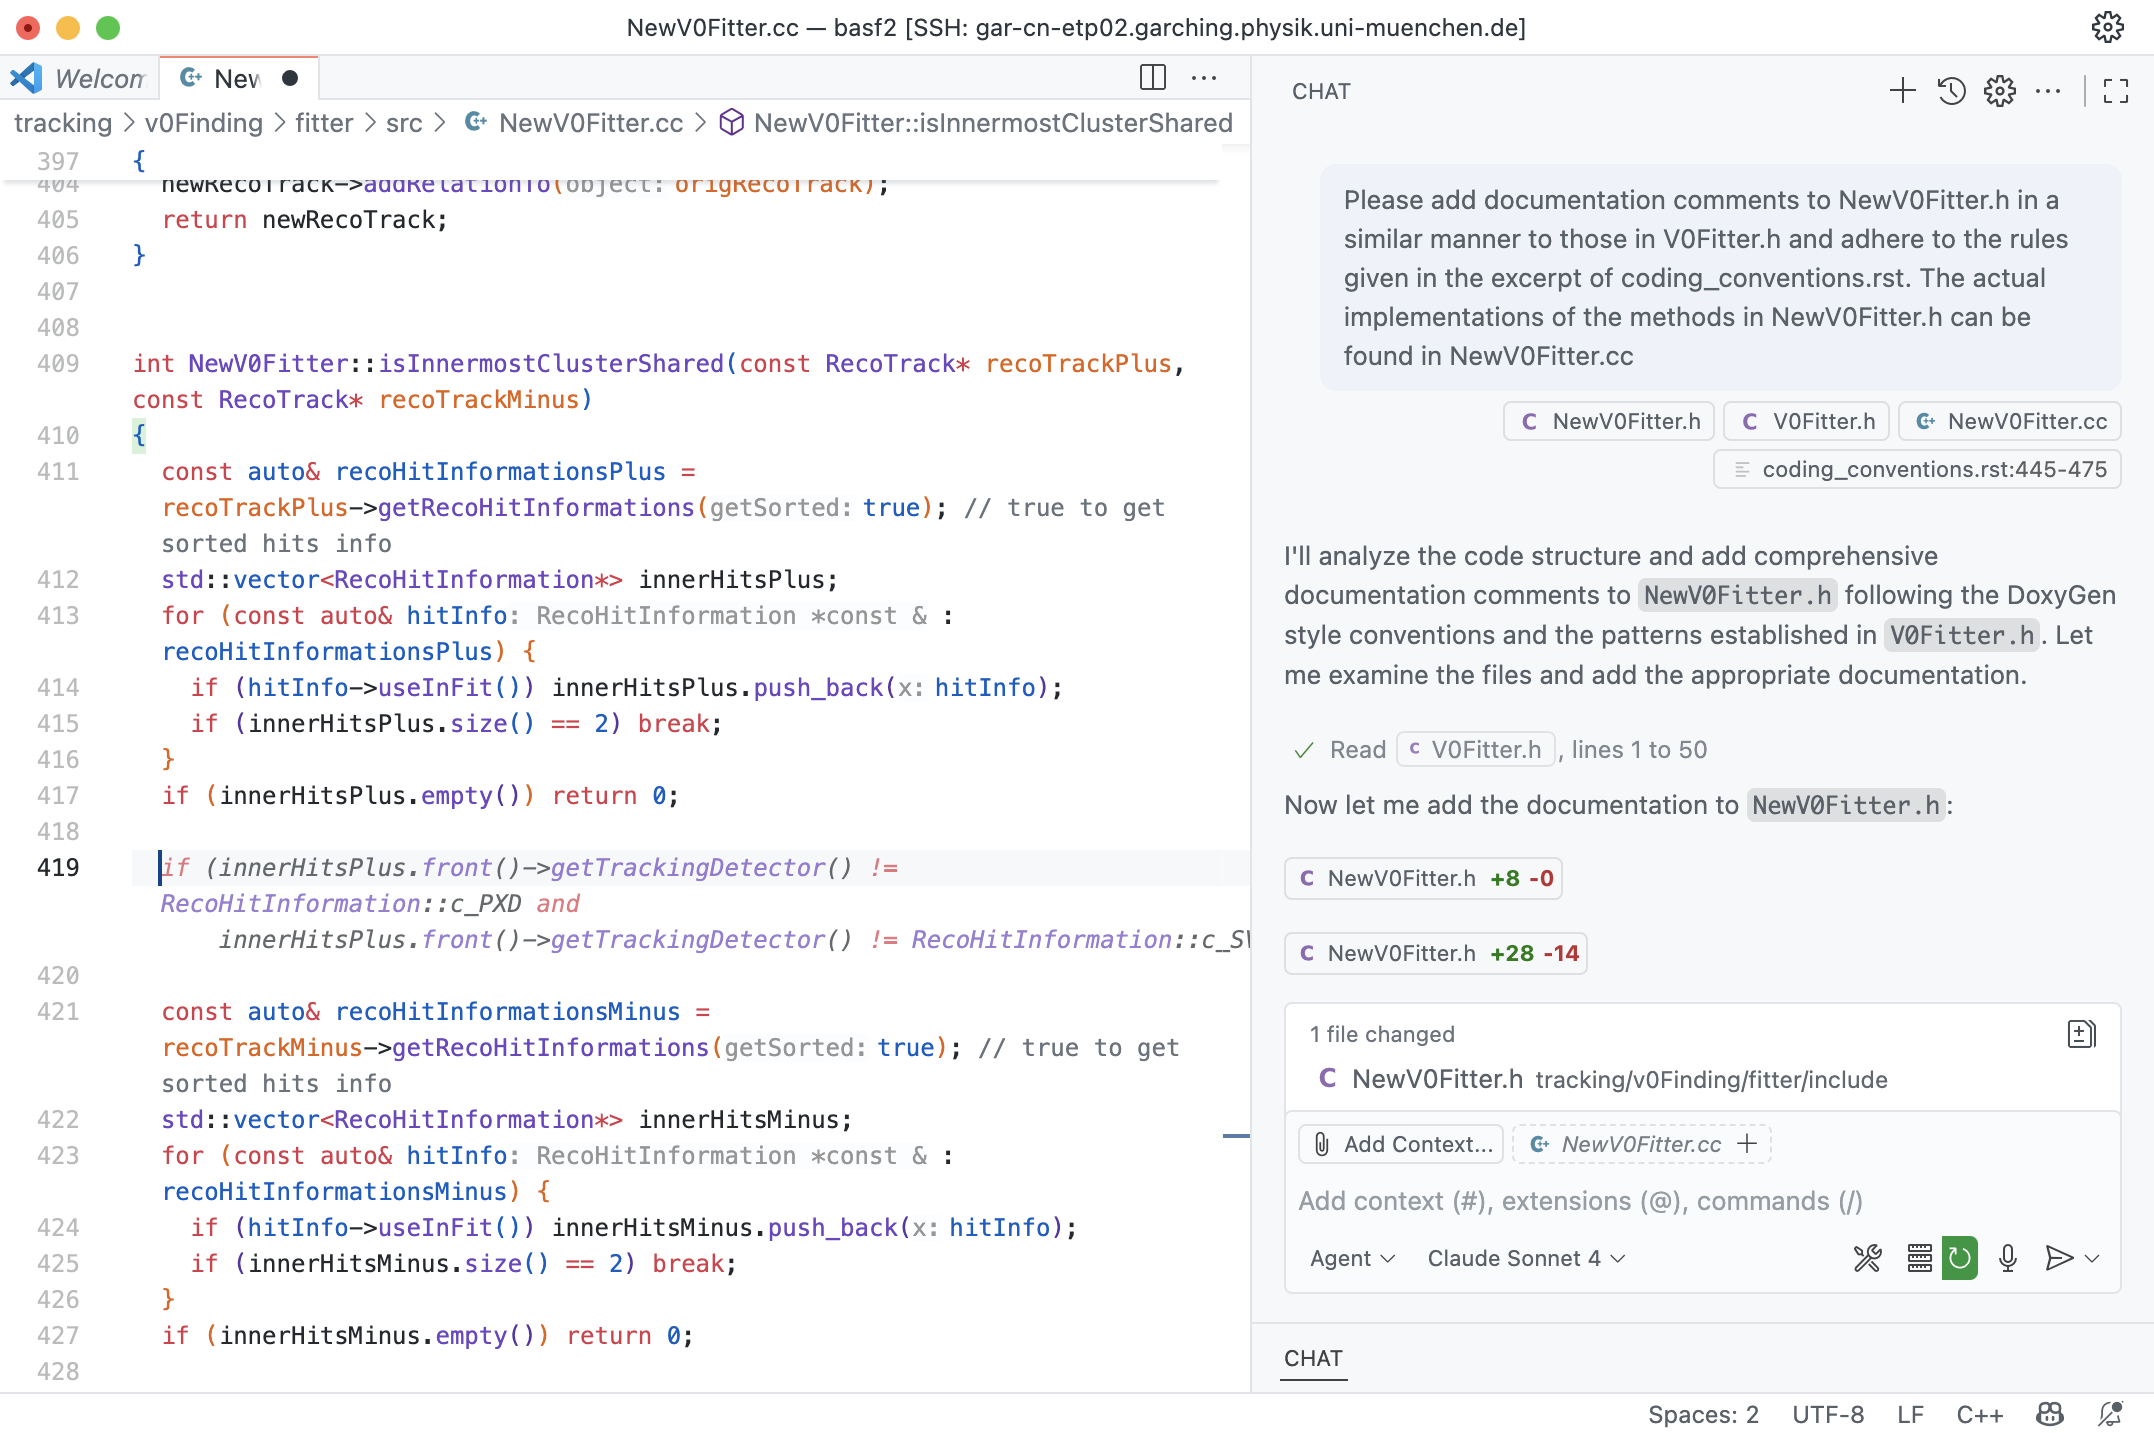
\includegraphics[width=0.9\textwidth]{static/vscode-copilot.png}
    \captionsetup{justification=raggedright,singlelinecheck=false}
    \caption{%
        GitHub Copilot integration in VS Code: \emph{Left}: code completion suggestion\\%
        \emph{Right}: Copilot panel with chat mode and model selection; message context is displayed beneath the text%
    }
    \label{fig:copilot-ui}
\end{figure}